\begin{frame}
\frametitle{Simics pipe}

\begin{columns}
  \column{0.5\textwidth}

  \begin{block}{Magic instructions}
    \begin{itemize}
    \item \dvtcmdcodeinline{nop} instruction
    \item Invokes callback function in Simics
    \item Low-latency
    \end{itemize}
  \end{block}

  \begin{block}{Implementation}
    \begin{itemize}
    \item Transmit buffer address in register
    \item Translate address using MMU
    \item Locate memory page(s) using physical address
    \end{itemize}
  \end{block}
  
  \column{0.5\textwidth}
  \begin{center}
    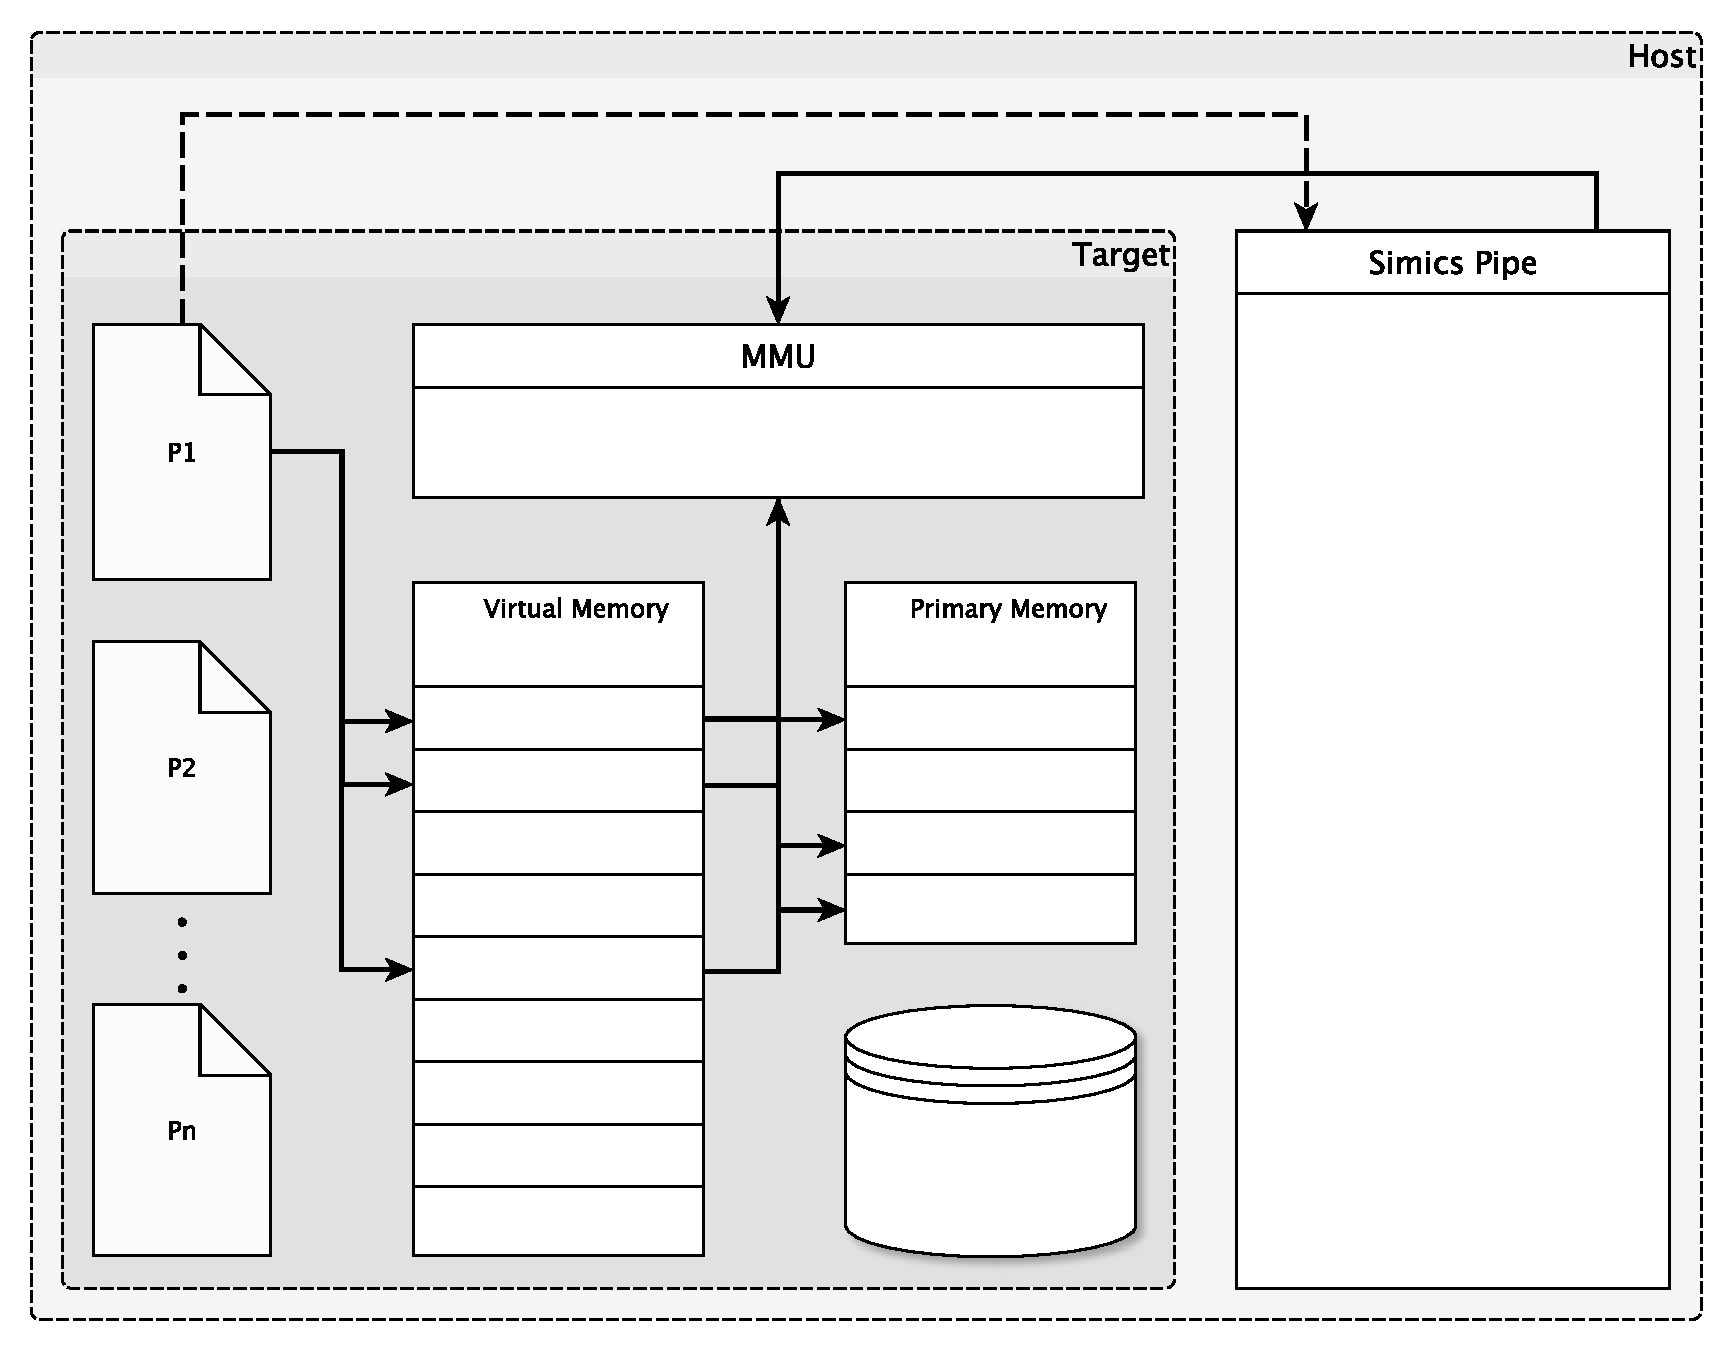
\includegraphics[height=0.5\textheight]{yedvirtualmemory.pdf}
  \end{center}
\end{columns}

\end{frame}
